\section{Trực quan hóa dữ liệu hướng thời gian}
Dữ liệu và thời gian đã được trình bày trong phần trước, tuy nhiên chúng ta cũng phải xem xét các vấn đề về thiết kế ở cấp độ biểu diễn trực quan. Để biểu diễn sự phụ thuộc vào thời gian của dữ liệu, ta cần đưa vào trục thời gian. Sự đa dạng của các kĩ thuật trực quan hóa bao gồm các cách tiếp cận rất khác nhau. Để tóm lược sự đa dạng này, chúng tôi tập trung vào 2 tiêu chí cơ bản:
\begin{itemize}
    \item \textit{Ánh xạ của thời gian}. Có hai lựa chọn cho ánh xạ thời gian: ánh xạ thời gian vào không gian và ánh xạ từ thời gian vào thời gian. Khi nói đến ánh xạ từ thời gian vào không gian, điều đó có nghĩa là thời gian và dữ liệu được thể hiện trong một hình ảnh duy nhất. Biểu diễn này không tự thay đổi theo thời gian, đó là lý do tại sao chúng tôi gọi đó là trực quan hóa dữ liệu hướng thời gian \textit{tĩnh}. Ngược lại biểu diễn \textit{động} sử dụng thời gian vật lý để truyền đạt sự phụ thuộc vào thời gian của dữ liệu, nghĩa là thời gian ánh xạ vào thời gian. Các kết quả này trong biểu diễn tự thay đổi theo thời gian (ví dụ bản trình chiếu hay hiệu ứng hoạt họa). Lưu ý rằng, có hay không sự tương tác để điều hướng thời gian không ảnh hưởng đến việc cách tiếp cận trực quan hóa là tĩnh hay động.
    \item \textit{Kích thước của không gian biểu diễn}. Chúng ta có thể phân biệt giữa biểu diễn 2D và 3D của dữ liệu hướng thời gian. Cách trực quan hóa sử dụng không gian 2D phải đảm bảo nhấn mạnh trục thời gian vì chiều thời gian và dữ liệu thường có chung biểu diễn sẵn có. Trong trường hợp biểu diễn 3D, chiều hiển thị thứ 3 được đưa vào. Thực tế, nhiều kĩ thuật sử dụng nó như một chiều dành riêng cho trục thời gian, tách thời gian ra khỏi các chiều dữ liệu khác một cách rõ ràng.
\end{itemize}
\subsection{Phân loại}
Để thuận lời cho việc phân loại một cách dễ dàng và giữ cho phân loại các kĩ thuật trực quan hóa đơn giản, chúng tôi tập trung vào những khía cạnh cốt lõi của dữ liệu, thời gian và trực quan hóa. Qua nhiều ví dụ trực quan hóa, chúng tôi sẽ minh họa những khả năng ứng dụng của chúng và những tính năng của các kĩ thuật trực quan hóa này.
\begin{itemize}
    \item \textbf{Dữ liệu} 
    \item[] \begin{itemize}
        \item \textit{Khung tham chiếu} - trừu tượng, không gian
        \item \textit{Các biến} - đơn biến, đa biến
    \end{itemize}
    \item \textbf{Thời gian}
    \item[] \begin{itemize}
        \item \textit{Sắp xếp} - tuyến tính, tuần hoàn
        \item \textit{Thời gian nguyên thủy} - thời điểm, khoảng
    \end{itemize}
    \item \textbf{Trực quan hóa}
    \item[] \begin{itemize}
        \item \textit{Ánh xạ} - tĩnh, động
        \item \textit{Số chiều} - 2D, 3D
    \end{itemize}
\end{itemize}
Để thiết lập những kĩ thuật trực quan hóa khác nhau cho dữ liệu hướng thời gian, chúng ta cần trả lời những câu hỏi sau:
\begin{itemize}
    \item \textit{Cái gì} được biểu diễn ? \textit{Thời gian và dữ liệu}
    \item \textit{Tại sao} nó được biểu diễn ? \textit{Tác vụ của người dùng}
    \item Nó được biểu diễn \textit{thế nào} ? \textit{Biểu diễn trực quan}
\end{itemize}
Trong chương này, chúng tôi chủ yếu nói về thời gian, dữ liệu và biểu diễn trực quan, bỏ qua những tác vụ của người dùng để mọi thứ trở nên dễ hiểu nhất có thể. Các kĩ thuật trực quan hóa đòi hỏi phải hiểu rõ những khâu cụ thể được thực hiện trong quá trình khai phá dữ liệu và trực quan hóa. MacEachen [281] đã đề xuất một phương pháp ở cấp độ thấp giả quyết một phần cụ thể trong miền thời gian. Các khâu này được định nghĩa bởi một tập các câu hỏi quan trọng mà người dùng có thể tìm kiếm câu trả lời bằng biểu diễn trực quan hóa, ví dụ như \textit{sự tồn tại của thành phần dữ liệu}: liệu thành phần này có tồn tại trong một thời điểm (khoảng) nào đó, hoặc là \textit{tốc độ thay đổi}: thành phần dữ liệu này thay đổi nhanh như thế nào theo thời gian. 
\\ \\
Trong phần tiếp theo, chúng tôi sẽ đưa ra các ví dụ cho mỗi loại được nêu trên.

\subsection{Dữ liệu: Khung tham chiếu - tóm lược}
KronoMiner [488] là một công cụ thăm dò chuỗi thời gian đa năng cung cấp khả năng điều hướng phong phú và hỗ trợ phân tích (hình (\ref{fig:f7.3})). Biễu diễn của nó dựa trên bố cục tâm phân cấp, cho phép người dùng có thể  quan sát chi tiết bằng cách tập trung vào các mảnh khác nhau. Các mảnh dữ liệu có thể được xoay, kéo, co dãn hoặc thu nhỏ một cách dễ dàng, hỗ trợ nhiều kiểu phân tích dữ liệu thời gian. KronoMiner cũng giới thiệu 2 kỹ thuật phân tích: (1) MagicAnalytics Lens, thể hiện mối tương quan của 2 thành phần dữ liệu xếp chồng lên nhau và (2) chế độ Best Match, trong đó một hình cung được hiển thị thể hiện sự tương tự của hai thành phần dữ liệu theo một phép đo cụ thể. 
\begin{figure}[H] % places figure environment here   
    \centering % Centers Graphic
    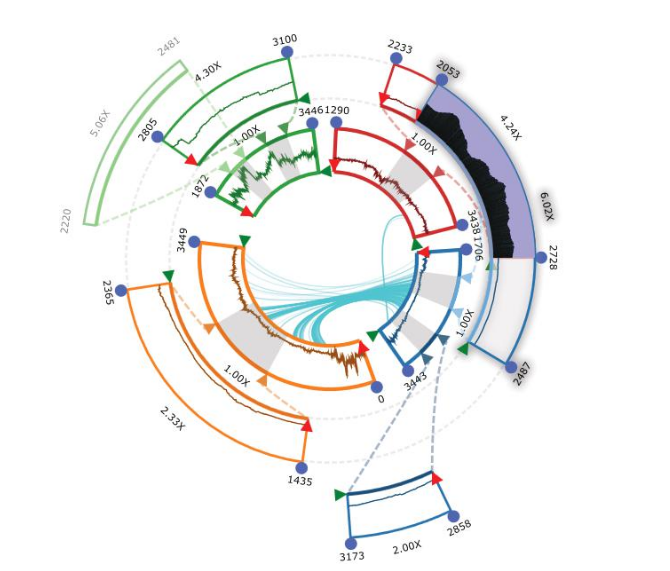
\includegraphics[width=1\textwidth]{assets/fig_7_3.png} 
    \caption{KronoMiner [488]. KronoMiner là một công cụ khám phá chuỗi thời gian đa mục đích cung cấp các tính năng điều hướng và phân tích phong phú} % Creates caption underneath graph
    \label{fig:f7.3}
\end{figure}
\subsection{Dữ liệu: Khung tham chiếu - Không gian}
Tominski và Schulz [415] giới thiệu kĩ thuật trực quan hóa cho dữ liệu thời gian có yếu tố không gian địa lý 2D và thời gian tuyến tính 1D. Ý tưởng là xây dựng một lát cắt không phẳng được gọi là \textit{Great Wall of Space-Time} (hình 7.4) thông qua không-thời gian liên tục 3D (2D+1D). Kiến trúc bức tường này được xây dựng dựa trên các khía cạnh tô tô và hình học của không gian địa lý. Dựa trên một đồ thị lân cận, một đường tô pô được thiết lập tự động hoặc có tương tác. Đường tô pô này được biến đổi thành đường địa lý thông qua những tính chất địa lý của khu vực trên bản đồ. Đường này được dựng thành một bức tường 3D mà chiều thứ 3 có thể được dùng để ánh xạ đến miền thời gian. Những biểu diễn trực quan khác nhau có thể được chiếu lên bức tường này để biểu thị dữ liệu. Bức tường có lợi thế là nó thể hiện một đường khép kín qua không gian mà không có khoảng trống giữa các pixel mang thông tin trên màn hình. 
\begin{figure}[H] % places figure environment here   
    \centering % Centers Graphic
    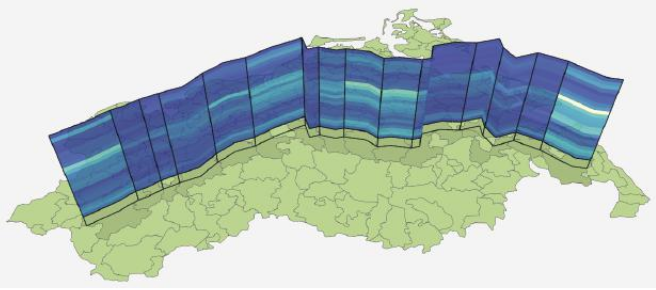
\includegraphics[width=1\textwidth]{assets/fig_7_4.png} 
    \caption{Biểu diễn trực quan hoa của dữ liệu sức khỏe con người sử dụng Great Wall of Space-Time. Một đường trong không gian được thiết lập. Dọc theo đường này, bức tường thể hiện 24 tháng của dữa lioeeuj tại mỗi vùng nó đi qua. Các màu tối thể hiện giá trị dữ liệu thấp, màu sáng thể hiện giá trị cao. Hình trên mô tả số ca mắc cúm } % Creates caption underneath graph
    \label{fig:f7.4}
\end{figure}
\subsection{Dữ liệu: Số biến - Đơn biến}
Trực quan hóa GROOVE (Granularity Overview OVErlay) [262] mở rộng trực quan hóa dựa trên pixel bằng cách phủ lên lớp tổng hợp một hoặc nhiều trong 3 phương pháp: (1) lớp phụ theo màu, (2) lớp phủ theo độ mờ hoặc (3) lớp phủ không gian. Các mức tổng hợp là kết quả của các mức độ chi tiết thời gian khác nhau. Các lớp phủ cho phép đọc vi mô và vĩ mô và trán chuyển động của mắt giữa việc quan sát tổng quan và chi tiết. Với mục đích mình họa, chúng tôi giữ sự hiển thị đơn giản và lượng dữ liệu trực quan không nhiều. Không gian trống xuất hiện do sự bất thường của việc kết hợp các chi tiết tuần và tháng. 
\\ \\
Đầu tiên, các thành phần màu có thể được sử dụng với lớp phủ màu (hình 7.5). Hình này vẽ sơ đồ dữ liệu lưu lượng trong vài tuần. 